\documentclass{standalone}

\usepackage{xcolor}

\definecolor{myblue}{HTML}{377EB8}
\definecolor{myred}{HTML}{E41A1C}

\usepackage{tikz}
\usepackage{pgfplots}
\pgfplotsset{compat=newest}

\usepackage{lmodern}
\SetSymbolFont{letters}{bold}{OML}{cmbr}{bx}{it}
\renewcommand{\familydefault}{\sfdefault}

\usepackage{sansmathfonts}

\begin{document}
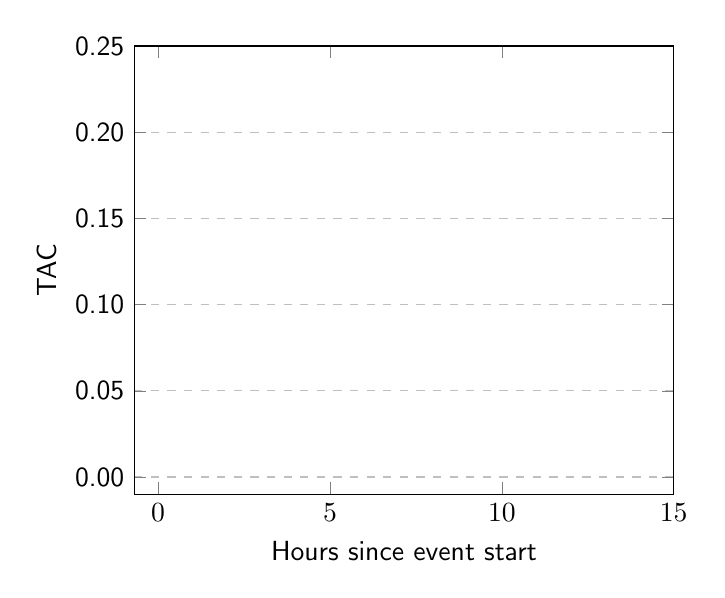
\begin{tikzpicture}
	\begin{axis}[
			xlabel={Hours since event start},
			ylabel={TAC},
			xmin=-0.70, xmax=15,
			ymin=-0.01, ymax=.25,
			xtick={0,5,10,15},
			ytick={0,0.05, 0.10,0.15,0.20,0.25},
			yticklabels={0.00,0.05, 0.10,0.15,0.20,0.25},
			ymajorgrids=true,
			grid style=dashed,
		]
						
		\addplot[
			color=myblue,
			mark=o,
		]
		coordinates {
            % (0, 0)
            % (0.5, 0)
            % (1.016666667, 0)
            % (1.516666667, 0)
            % (2.033333334, 0)
            % (2.55, 0)
            % (3.05, 0)
            % (3.566666667, 0)
            % (4.083333334, 0)
            % (4.583333334, 0)
            % (5.1, 0)
            % (5.6, 0)
            % (6.116666667, 0)
            % (6.633333334, 0)
            % (7.2, 0)
            % (7.716666667, 0)
            % (8.233333334, 0)
            % (8.733333334, 0)
            % (9.233333334, 0)
            % (9.766666667, 0)
            % (10.28333333, 0)
            % (10.76666667, 0)
            % (11.3, 0)
            % (11.81666667, 0)
            % (12.31666667, 0)
            % (12.81666667, 0)
            % (13.33333333, 0)
            % (13.83333333, 0)
            % (14.33333333, 0)
            % (14.83333333, 0)
            % (15.33333333, 0)
            % (15.83333333, 0)
		};
	\end{axis}
\end{tikzpicture}
\end{document}
